\subsection{Bounds on \texorpdfstring{$\lambda_m$}{lambda m} and the (higher) derivatives of \texorpdfstring{$\phi$}{phi}}
\label{sec:smooth}


Estimating and uniformly bounding the $k$-th derivative of $\phi$,
$\|d^k\varphi\|$, plays an important role in controlling other
geometric quantities such as $\tau_{min}$ and proving existence of
local one--to--one parametrization of $\varphi(\mathcal{M})$. Recall that $k$ is the smoothness of $\MM$. Because the $i$--th component of map $\varphi:M \rightarrow \mathbb{R}^m$
is $e_i$ multiple of $e^{-\lambda_i t_0/2}$ which is a bounded scalar when $t_0$ is fixed, we can ignore
it when we estimate the upper bound.

We notice that $\varphi(M)$ is a $d$--dimensional manifold embedded in $\mathbb{R}^m$, then $d\varphi_p$ is a map such that 
\begin{align}
	d\varphi_p:T_p M \rightarrow T_{\varphi(p)}\varphi(M)\hookrightarrow\mathbb{R}^m
\end{align} 
and we can treat the tangent vector in $\mathbb{R}^m$ as a tangent vector in $T_\varphi(p) \varphi(M)$ through the natural isomorphism. This isomorphism maps local basis to local basis, thus this map is also isometric. In the following, we will consider $T_{\varphi(p)} \varphi(M) \cong \mathbb{R}^d$ and $T_{\varphi(p)} \varphi(M) \subset \mathbb{R}^m$ as equivalent through this mapping.
%
\begin{figure}[H]
	\centering
	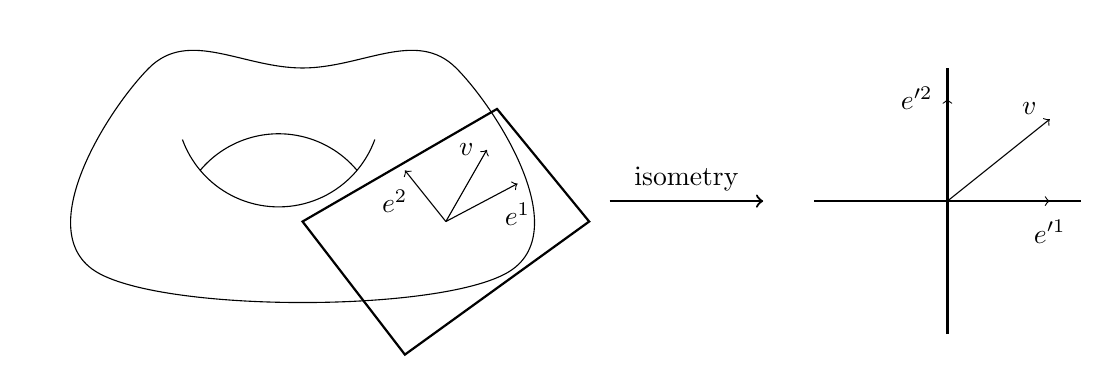
\begin{tikzpicture}[scale=1.3]
		\draw[smooth cycle,tension=.7] plot coordinates{(0,0) (0.5,2) (2,2) (3.5,2) (4,0)};
		\coordinate (A) at (1,1);
		\draw (A) arc(140:40:1) (A) arc(-140:-20:1) (A) arc(-140:-160:1);
		
		
		\draw[thick] (2,0.5) -- (3,-0.8) -- (4.8,0.5) -- (3.9,1.6) -- cycle;
		% 标注e1和e2
		\draw[->] (3.4,0.5) -- (4.1,0.87);
		\draw[->] (3.4,0.5) -- (3.0,1);
		\node at (4.1,0.57) {\(e^1\)};
		\node at (2.9,0.7) {\(e^2\)};
		
		% 标注v向量
		\draw[->] (3.4,0.5) -- (3.8,1.2);
		\node at (3.6,1.2) {\(v\)};
		
		% 等距映射箭头
		\draw[->, thick] (5,0.7) -- (6.5,0.7) node[midway, above] {isometry};
		
		% 绘制右侧的欧几里得平面
		\draw[thick] (7,0.7) -- (9.6,0.7);
		\draw[thick] (8.3,-0.6) -- (8.3,2);
		
		% 标注e1'和e2'
		\draw[->] (8.3,0.7) -- (9.3,0.7);
		\draw[->] (8.3,0.7) -- (8.3,1.7);
		\node at (9.3,0.4) {\(e'^1\)};
		\node at (8.0,1.7) {\(e'^2\)};
		
		% 标注v'向量
		\draw[->] (8.3,0.7) -- (9.3,1.5);
		\node at (9.1,1.6) {\(v\)};
		
	\end{tikzpicture}
	\caption{Isometry}
\end{figure}
%



\subsubsection{Upper Bound of \texorpdfstring{$\lambda_m$}{lambda\_m}}
\label{sec:phim-lambdam}


The most classical result for estimating eigenvalues is Weyl's law:
\begin{align}
N(\lambda)\sim \frac{\omega(d) Vol(M) \lambda^\frac{d}{2}}{(2\pi)^{d}},
\end{align}
where $N(\lambda)$ is the number of eigenvalues less than or equal to $\lambda$. 

If we ask $\lambda=\lambda_k$, the above is equivalent to
\begin{align}
	\lambda_k^{d/2} \sim \frac{(2\pi)^d k}{\omega(n) Vol(M)}
\end{align}

Weyl's law provides an asymptotic expression for the eigenvalues of the Laplace--Beltrami operator, offering profound insights into their growth rates. However, in our paper, strict control for eigenvalues is essential. This requires not only asymptotic estimates but also rigorous upper bounds that hold universally. A notable result for the upper bound was established by Li--Yau \cite[Thm. 16]{esteigenvalue}, who derived explicit upper bounds for the eigenvalues under geometric constraints, which align with the assumptions in our study.


We estimate the upper bound of eigenvalues. If the lower bound of the Ricci curvature $\kappa_M$ of $M$ is less than $0$, we have 
\begin{align}
	\lambda_k \leq 
	\left\{
	\begin{array}{l}
		\displaystyle \frac{(2\beta+1)^2}{4}(-\kappa_M) + 4(1+2^\beta)^2\pi^2 \left(\frac{\sinh \sqrt{-\kappa_M}\text{diam}}{\sqrt{-\kappa_M}\text{diam}}\right)^\frac{2d-2}{d} \\
		\hspace{10em} \times \left((k+1)\frac{\alpha(d-1)}{d}\frac{1}{V}\right)^\frac{2}{d} \\[1.5ex]
		\text{when } d=2(\beta+1), \beta = 0,1,2\dots \\[2.5ex]
		\displaystyle \frac{(2\beta+2)^2}{4}(-\kappa_M) + 4(1+\pi^2)(1+2^{2\beta})^2 \left(\frac{\sinh \sqrt{-\kappa_M}\text{diam}}{\sqrt{-\kappa_M}\text{diam}}\right)^\frac{2d-2}{d} \\
		\hspace{10em} \times \left((k+1)\frac{\alpha(d-1)}{d}\frac{1}{V}\right)^\frac{2}{d} \\[1.5ex]
		\text{when } d=2\beta+3, \beta = 0,1,2\dots
	\end{array} 
	\right. ,
\end{align}


if $M$ has non--negative Ricci curvature $\kappa_M$, we have
\begin{align}
	\lambda_k \leq (d+4)d^{1-\frac{2}{d}}\left(\frac{k+1}{V}\alpha(d-1)\right)^\frac{2}{d} ,
\end{align}
where $d$ is the dimension of $M$, $V$ is the volume of $M$ and $\alpha(n)$ is the volume of $S^n$ in $\mathbb{R}^{n+1}$.\cite{esteigenvalue}

Since for $M \in \mathcal{M}$, the volume is greater that $V_1$ and the lower bound of the Ricci curvature is greater than $\kappa$, so $\frac{1}{V}\leq \frac{1}{V_1}$ and $-\kappa_M\leq -\kappa$, thus we have 
\begin{align}
	\lambda_k \leq \left\{
	\begin{array}{cc}
		C(d,V) (k+1)^\frac{2}{d} \quad &\text{if } \kappa_M \text{ is non-negative} \\
		C(d,\kappa,\text{diam},V) (k+1)^\frac{2}{d} \quad  &\text{if } \kappa_M \text{ is negative}
	\end{array}
	\right. .
\end{align}
Summarizing above, we have
	\begin{lemma}[Uniform upper bound on $\lambda_k$]
	\label[lemma]{lem:lambdam-bound}
	There exists a constant $C(\MM)$, depending only on the uniform geometric parameters $(d,\kappa,\mathrm{diam},V)$ of the family $\MM$, such that
	\begin{align}
		\lambda_k \leq C(\MM) (k+1)^\frac{2}{d} \qquad \text{for all } M \in \MM.
	\end{align}
\end{lemma}



\subsubsection{Estimate of Higher Order Derivatives}
\label{sec:phim-higher-deri}

In this subsection, we will estimate the $L^\infty$ norm of higher order derivatives for eigenfunctions to control the operator norm of $d N^\prime$ in the next subsection.  

One similar result is Bernstein inequality, for eigenfunction $e_\lambda$ of $\Delta$: $\Delta e_\lambda =\lambda e_\lambda$, we have\cite{xu2009gradient}:
\begin{align}
	\|\nabla e_\lambda\|_{L^\infty}\leq C\lambda^{\frac{1}{2}} \|e_\lambda\|_{L^\infty}
\end{align}


\cite{xu2005asymptotic} proved a more general estiamte, for eigenfunction $e_\lambda$ of $\Delta$: $\Delta e_\lambda =\lambda e_\lambda$, we have 
\begin{align}
	\|e_\lambda\|_{H^\infty_k}\sim \lambda^\frac{k}{2} \|e_\lambda\|_{L_\infty} \quad \text{as }\lambda \rightarrow \infty
\end{align}
where $\sim$ means the equivalence between two norms, and $\|\cdot\|_{H^k_\infty}$ is Sobolev norm. If we revise this result to have a upper bound (the author says we only need a little effort to do so), we can control $\|d^k \varphi\|$ since we have had the upper bound of $\lambda_m$ which only depend on $M$.

\cite{2004Xuhigherorder} also gave a better estimate:
\begin{align}
	\|e_\lambda(x)\|_{H^\infty_k} \leq C \lambda^{k/2+(d-1)/4}\|e_\lambda(x)\|_{L^2}
\end{align}
however, $C$ may not be an uniform constant for $M \in \mathcal{M}$.


To estimate the $L^\infty$ norm of derivatives for eigenfunctions, we first choose the coordinate chart to be normal coordinate chart to make our derivatives well defined. We take derivative of $e(x): M \rightarrow \R$ in the following sense: Let $x \in U$ be the normal coordinate chart $(U,\textbf{x})$ and $\hat{U}=\textbf{x}(U)$, then $\hat{e}(x)=e\circ \textbf{x}^{-1}:\hat{U}\rightarrow R$ be the coordinate representation of $e(x)$. We treat $\partial_i e(x)$ as $\partial_i \hat{e}(x)$, and for higher order derivatives as well.

\begin{lemma}[Uniform bound on the higher derivatives of the eigenfunctions]
	\label[lemma]{lem:eigfn-deri-bound}
	For every multi--index $\alpha$ with $|\alpha| \leq k$ there exists a constant $C_\alpha$, depending only on $\alpha$ and the uniform geometric parameters of $\MM$, such that the eigenfunction derivatives satisfy the pointwise bound
	\begin{align}
		|\partial^\alpha e_\lambda(x)| \leq C_\alpha (1+\lambda)^{k/2+d/4}, \qquad |\alpha| \leq k.
	\end{align}
\end{lemma}
 Consequently, since $\lambda_k$ is bounded above by $C(\MM)(k+1)^\frac{2}{d}$, $\varphi_j = (2t)^\frac{d+2}{4}\sqrt{2}(4\pi)^\frac{d}{4}e^{-\lambda_1 t}e_j(x)$, then the coordinate derivatives of $\varphi$ up to order $k$ are uniformly bounded over $M \in \MM$.

\begin{proof}[Proof of \cref{lem:eigfn-deri-bound}]
Let $\gamma$ be a $2d$ multi--index with $|\gamma|:=\sum_i\gamma_i\leq k$, and $x,y \in U$ be a geodesic normal coordinate of $M$. We denote $\sum_{\lambda_j\leq \lambda} e_j(x) e_j(y)$ as $e(x,y,\lambda)$. Let $\gamma = \left(\gamma_1,\dots,\gamma_{2d}\right)$, then the $\gamma$ order derivative for $e_j(x) e_j(y)$ is 
\begin{align}
	\partial^\gamma_{x,y} e_j(x) e_j(y) = \frac{\partial^{|\gamma_1+\cdots+\gamma_{d}|}e_j(x)}{\partial x_1^{\gamma_1} \cdots \partial x_d^{\gamma_d}} \frac{\partial^{|\gamma_{d+1}+\cdots+\gamma_{2d}|}e_j(y)}{\partial y_1^{\gamma_{d+1}} \cdots \partial y_d^{\gamma_{2d}}}
\end{align}

We have \cite[Lem. 2.4]{2004Xuhigherorder}
\begin{align}
	|\partial^\gamma_{x,y}e(x,y,\lambda)|\leq C_\gamma (1+\lambda)^{\frac{d+|\gamma|}{2}}.
\end{align}

To have the estimate for derivatives of eigenfunctions, let $\alpha$ be a $d$ dimension multi--index, and using the inequality above with $\gamma = \left(\alpha , \alpha\right)$, then we have 
\begin{align}
	|\partial^\alpha e_\lambda (x)|^2\leq\sum\limits_{\lambda_j\leq \lambda} |\partial^\alpha e_j(x)|^2 \leq C_\alpha (1+\lambda)^{d/2+|\alpha|}
\end{align}
so
\begin{align}
	\label{deriinequ}
	\|e_\lambda\|_{H^\infty_k}=\max\limits_{|\alpha|\leq k}|\partial^\alpha e_\lambda(x)|\leq \sup\limits_{|\alpha|\leq k}\left\{C_\alpha\right\}(1+\lambda)^{k/2+d/4}
\end{align}
Since $\lambda_k$ is bounded above by $C(\MM) (k+1)^{\frac{2}{d}}$, which implies that $\|\varphi_j\|_{H_k^\infty}\leq C(l)$ for $\varphi_j:M \rightarrow \mathbb{R}$. Therefore, $|\frac{\partial^l \varphi_j}{\partial x_{i_1}\cdots\partial x_{i_l}}| \leq C(l)$ for $l\leq k$ with respect to normal coordinate.
\end{proof}

After deriving the uniform bound for the norm of the derivatives of $\phi$, we now establish the bound of the operator norm of the covariant derivatives.
\begin{lemma}[Uniform bound on the higher derivatives of the embedding map $\varphi$]
	\label[lemma]{lem:covar-deri-bound}
	For every $l \leq k$ there exists a constant $A(l)$, depending only on $l$ and the uniform geometric parameters of $\MM$, such that the operator norm of the $l$-th derivative of the embedding map is bounded uniformly over $\MM$:
	\begin{align}
		\|d^l \varphi\| \leq \sqrt{m}\,A(l)\,d^{l/2} \quad \text{for all }M \in \MM.
	\end{align}
\end{lemma}

\begin{proof}[Proof of \cref{lem:covar-deri-bound}]
By \cref{lem:eigfn-deri-bound}, the coordinate derivatives of $\varphi$ up to order $k$ are uniformly bounded over $M \in \MM$; we use this together with the uniform bounds on the Christoffel symbols and their derivatives to control $\|d^l\varphi\|$.

To estimate the norm of $d\varphi$, we can derive its local coordinate representation and compute the covariant derivatives in the normal chart since  choosing different chart does not have the influence on the norm. Now we denote $\varphi$ as $j$--th component of $\varphi$ to simplify the notation and let $(U,\textbf{x})$ be the normal chart.

For the first order covariant derivative, we have
\begin{align}
	\nabla \varphi (X) = \nabla_X \varphi = X\varphi,
\end{align} 
thus 
\begin{align}
	\nabla \varphi = \varphi_i dx^i\quad  \text{with}\ \varphi_i = \partial_i \varphi,
\end{align}
so for the first order covariant derivative, the local coordinate representation is the first order derivative of local representation of $\varphi$.

For second order covariant derivative, which is also known as covariant Hessian. We have 
\begin{align}
\nabla^2 \varphi (X,Y)= \nabla^2_{Y,X}=\nabla_Y(\nabla_X \varphi)-\nabla_{\nabla_Y X}\varphi=X(Y\varphi)-(\nabla_X Y)\varphi
\end{align}
thus in local coordinates,
\begin{align}
	\nabla^2 \varphi = \varphi_{ij} dx^i \otimes dx^j \quad \text{with}\ \varphi_{ij}=\partial^2_{ij}\varphi-\Gamma^k_{ij}\partial_k \varphi,
\end{align}
%
with $i,j,k\in\{1,2,\ldots d\}$. 
For the third order coordinate derivative, we have 
\begin{align}
	\nabla^3 \varphi (X,Y,Z)&=(\nabla_Z \nabla^2 \varphi) (X,Y)\\
	&=Z(\nabla^2 \varphi (X,Y))-\nabla^2\varphi (\nabla_Z X,Y)-\nabla^2 \varphi (X,\nabla_Z Y)\\
	&=Z(X(Y\varphi)-(\nabla_X Y)\varphi)-\nabla_Z X(Y\varphi)+(\nabla_{\nabla_Z X} Y)\varphi \nonumber \\
	&\qquad\qquad \quad -X(\nabla_Z Y\varphi)+(\nabla_X \nabla_Z Y)\varphi,
\end{align}
thus in the local coordinate, 
\begin{align}
 \nabla^3 \varphi =\varphi_{ijk} dx^i \otimes dx^j \otimes dx^k &\\
 \text{with}\quad \varphi_{ijk}=\partial^3_{ijk} \varphi- \partial_k \Gamma_{ij}^l \partial_l \varphi - \Gamma_{ij}^l \partial^2_{kl}\varphi-\Gamma_{ik}^m\partial^2_{mj} \varphi&+ \Gamma_{ik}^l \Gamma_{lj}^m \partial_m \varphi-\partial_i \Gamma_{jk}^l \partial_l \varphi \nonumber\\
 & -\Gamma_{jk}^l \partial^2_{il}\varphi+ \Gamma_{il}^m\Gamma_{jk}^l\partial_m \varphi.
\end{align}

The local coordinate representation is combined with derivative of Christoffel symbol and third order derivative of $\varphi$. And we can prove easily by induction that the local coordinate representation of $\nabla^l \varphi$ is $\varphi_{i_1\cdots i_l} dx^{i_1} \otimes \cdots \otimes dx^{i_l}$
with $\varphi_{i_1\cdots i_l}$ can be represented by derivative of $\varphi$ not higher than order $l$ and derivative of Christoffel symbol not higher than order $l-2$. To prove this, we only need to notice that 
\begin{align}
	\nabla^{l+1}\varphi(X_1,\cdots,X_l,X)&=\nabla(\nabla^l \varphi)(X_1,\cdots,X_l,X) \\
	&=(\nabla_X \nabla^l \varphi) (X_1,\cdots,X_l)\\
	&=X(\nabla^l \varphi(X_1,\cdots,X_l))-\sum_{i=1}^l \nabla^l\varphi(X_1,\cdots,\nabla_X X_i,\cdots,X_l)
\end{align}

Since we assume for any $M \in \mathcal{M}$, the local coordinate
representation in the normal chart of the Christoffel symbols and
their derivatives with order not above $k-2$ have an uniform bound only depends on its order,
and we have claimed derivatives of $\varphi$ which order is not higher
than $k$ have an uniform bound, and we notice that the local
representation of $\nabla^k \varphi$ is combined with them in the same
pattern among all $M \in \mathcal{M}$. Therefore, $\varphi_{i_1\cdots
  i_l}$ is bounded uniformly for all $l \leq k$, i.e.
\begin{align}
|\varphi_{i_1\cdots i_l}| \leq A(l) \quad \text{for }l\leq k
\end{align}


With this control of upper bound, we can estimate the norm of higher derivatives of $\varphi$:
\begin{align}
	\|d^l \varphi\|&=\sup\limits_{\|v_1\|=1, \dots,\|v_l\|=1} \|\nabla^l \varphi (v_1,\dots,v_l)\| \\
	&=\sup\limits_{\|v_1\|=1, \dots,\|v_l\|=1} \|\nabla^l \varphi (v_1\otimes\dots\otimes v_l)\| \\
	&=|\varphi_{i_1\cdots i_l} dx^{i_1} \otimes \cdots \otimes dx^{i_l} (v_1^{i_1} \frac{\partial}{\partial x^{i_1}} \otimes \cdots \otimes v_l^{i_l} \frac{\partial}{\partial x^{i_l}})|\\
	&=|\varphi_{i_1\cdots i_l} v_1^{i_1} \cdots v_l^{i_l}| \\
	&\leq A(l) \left|\sum_{i_1,i_2,\dots i_l=1}^d   v_1^{i_1} \cdots v_l^{i_l}\right|\\
	&= A(l) \left|\sum_{i_1=1}^{d} v_1^{i_1} \sum_{i_2,\dots i_l=1}^dv_2^{i_2} \cdots v_l^{i_l}\right|\\
	\text{(AM-–GM)}&\leq A(l) \left|\sum_{i_2,\dots i_l=1}^dv_2^{i_2} \cdots v_l^{i_l}\right| \sqrt{d}\\
	&\ \ \vdots \\
	&\leq A(l) d^{l/2}.
\end{align}

This inequality holds for all $l \leq k$. Here $\varphi : M \rightarrow \mathbb{R}$, thus $d^l \varphi (v_1,\dots,v_l)$ gives a vector in $\mathbb{R}$, and then $d^l \varphi (v_1,\dots,v_l) = \left(d^l\varphi_1(v_1,\dots,v_l),\dots,d^l\varphi_m (v_1,\dots,v_l)\right)$ is a vector in $\mathbb{R}^m$, which is also a tangent vector in $T_{\varphi(p)}\varphi(M)$ through the natural isometry. Since $d^l \varphi(v_1,\dots,v_l)$ has $m$ components, it is easy to check the operator norm of $d^l \varphi$ has the upper bound $\sqrt{m}A(l)d^{l/2}$. Therefore, $\|d^l \varphi\|$ are bounded uniformly for $l \leq k$.
\end{proof}